\chapter{Cryptocurrencies}

There were hundreds of failed attempts of creating cryptographic payment systems before cryptocurrencies like Bitcoin and Ethereum come into existence. Some of these systems are listed in figure \ref{paymentSystems}. All of them were created before Bitcoin, and despite that, some of these attempts were only academic proposals, others were actually deployed and tested systems, only a few of them survived to these days. One of the survival is PayPal, but only because it quickly give up its original idea of hand-held devices for cryptographic payments.\cite{wayner1997digital}

So there is a question, what makes cryptocurrencies successful nowadays?  It may be it's easy to use principle and no need for external hardware. 
Another critical component of cryptocurrencies discussed in this work is Blockchain. Simply, it is a ledger in which are all transactions securely stored. The idea behind blockchains is pretty old, and it was originally used for timestamping digital documents.\cite{haber1990time} 


\begin{figure}[h]
    \centering
    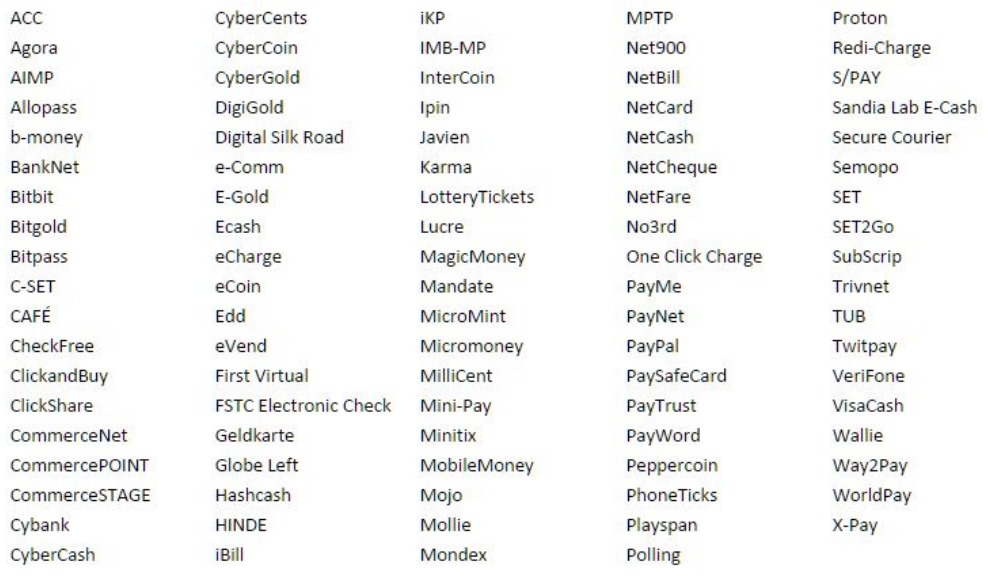
\includegraphics[width=14cm]{failedCryptos.PNG}
    \caption{Electronic payment systems before cryptocurrencies \cite{narayanan2016bitcoin}}
    \label{paymentSystems}
\end{figure}


\section{Bitcoin}
Bitcoin is probably the most famous cryptocurrency. On 3th January 2009, Satoshi Nakamoto (an alias for person or group persons authored the bitcoin white paper) minned the genesis block of bitcoin (block with height 0). Satoshi get reward of 50 bitcoins (half a million US dollars in the time of writing). This text was embedded in this coinbase transaction (see \ref{genesisBitcoin}): \textit{The Times 03/Jan/2009 Chancellor on brink of second bailout for banks.}\footnote{\url{https://en.bitcoin.it/wiki/Genesis\_block}}\cite{newYorkerBTC}. 

\begin{figure}[h]
    \centering
    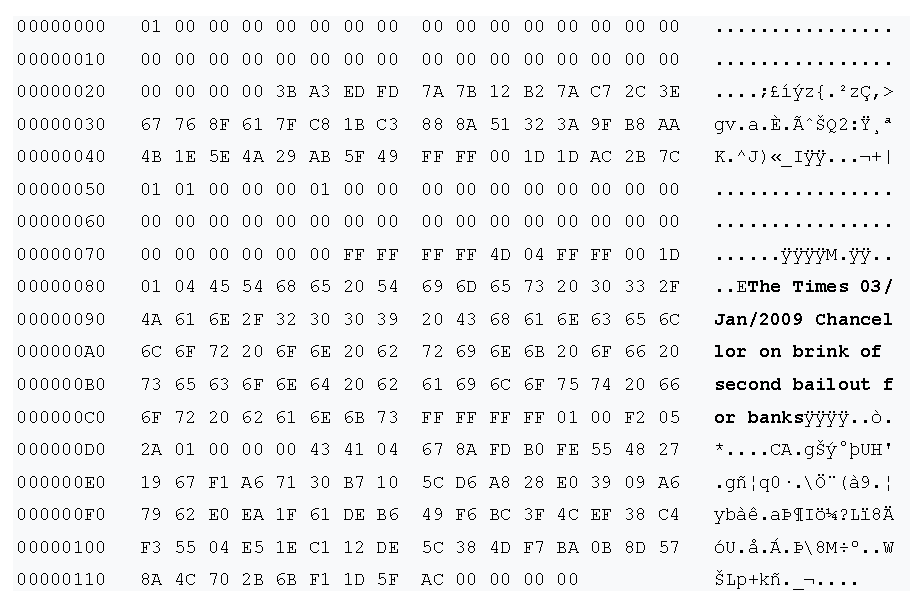
\includegraphics[width=14cm]{genesisBitcoin.pdf}
    \caption{Genesis bitcoin block}
    \label{genesisBitcoin}
\end{figure}

First documents purchase happend in 22nd May 2010, when Laszlo Hanyecz bought 2 pizzas for 10 000 bitcoins (\$41 then, now about \$80 000 000)\footnote{\url{https://bitcointalk.org/index.php?topic=137.0}}. This transactions hash is \texttt{a1075db55d416d3ca199f55b6084e\-2115b9345e16c5cf302fc80e9d5fbf5d48d} and will be stored in bitcoin blockchain forever. Actual photo of \$80 000 000 pizza is on figure \ref{bitcoinPizza}. 

\begin{figure}[h]
    \centering
    
\includegraphics[width=7cm]{btcPizza.jpg}
    \caption{Pizza for 10 000BTC}
    \label{bitcoinPizza}
\end{figure}


\section{DigiByte}
DigiByte was developed and released in 2013. It is based on Bitcoin with some adjustment in the code to improving functionality. In the late 2017 there were 200 000 pending transaction in Bitcoin. Minners were preffering transaction with bigger fee, so to confirm transaction, you needed to pay \$50. Digibyte solved this problem by adding new block every 15 seconds (new block in Bitcoin is minned every 10 minutes). Average transaction occupies 570 bytes of data. One black can contain approximaly 3 500 transactions given the 2 MB limit. This means that in DigiByte 500 transactions can be confirmed in one second compared to Bitcoin 4-7 transaction per second. DigiByte has also 1000:1 DigiByte to Bitcoin ratio so for every Bitcoin there will be 1000 DigiByte.


\section{Ethereum}
While both the Bitcoin and Ethereum networks are powered by the principle of distributed ledgers and cryptography, the two differ technically in many ways. For example, transactions on the Ethereum network may contain executable code, while data affixed to Bitcoin network transactions are generally only for keeping notes. Other differences include block time (an ether transaction is confirmed in seconds compared to minutes for bitcoin) and the algorithms that they run on (Ethereum uses ethash while Bitcoin uses SHA-256). 



\section{Decred}
Decred is cryptocurrency build from Bitcoin. Main difference from Bitcoin is rewarding system from minning. In Bitcoin, if minner that minned block will get full reward. This causes the blockchain to split when two or more miners fund a block at nearly the same time. The fork is resolved when subsequent block(s) are added and one of the chains becomes longer than the alternative(s). In Decred the chance of blockchain forks are minimized by  hybrid proof of work and proof of state system. Each time a block is created (by a miner), which is then approved by ticket holders, the miner receives a block reward (newly created DCR). If the block is rejected by ticket holders, the miner does not receive a reward. Tickets holders for new block are choose randomly. The ticket validates the previous block. A block needs at least 3 of the 5 votes chosen to approve it for it to be validated. This means that miners create the blocks, but they have to be approved by the stakeholders. This has many implications, including making a 51\% hashpower attack very difficult, and making a minority fork very difficult as well.

\section{Monero}
Three years after Bitcoin, in 2012, the competing Bytecoin cryptocurrency entered the market. The problem with this cryptocurrency, however, was that 80\% of all coins were mined in advance by its authors. The chances of mining were therefore not balanced. This led to the decision that this cryptocurrency would start again. It saw the light of day 18 April 2014 and was called BitMonero, a composite of the word coin in Esperanto (Monero) and Bitcoin according to Bitcoin. But after five days, the community decided to use only Monero for short.
